\subsection{Image classification using Convolutional Neural Networks }
As one of the biggest contributing factor to the rise of Deep learning, Convolutional neural network(CNN) (LeCun et al., 1998) has become the most dominant player in the field of image classification. The interest in CNN started with Alexnet(2012)\cite{CNN} which scored a top-5 accuracy of 15.3\% on the ImageNet competition\cite{ILSVRC15}, which was 10.8 percentage points lower than that of the runner up. Since then, the architecture of CNN has changed a lot, with deeper and more powerful performance. 
\begin{figure}[ht]
\begin{center}
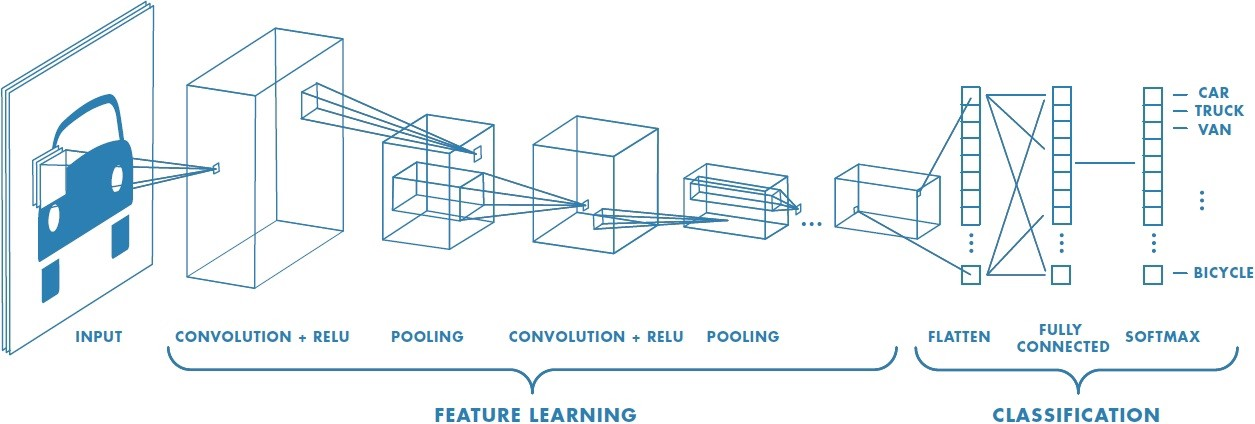
\includegraphics[width=0.5\columnwidth]{Image/CNN.jpeg}
\caption[CNNpic1]{ Basic convolutional neural network architecture \cite{CNNpic}}
\label{fig:BoxesAndArrowsAreNice}
\end{center}
\end{figure}

In short, convolutional networks are a subset of neural networks, they are also made up of neurons that have learnable weights and biases. In CNN, the network will process the input train data through a series of convolution layers with filters (Kernals), Pooling, fully connected layers (FC), etc... and then perform the classification with help of function like softmax at the end.\cite{CNN} Convolution in this case is the first layers of the network, which apply filters to the input tensor. It can extract the features from the image by preserving the relation between pixels. The pooling layer then use to reduce the numbers of parameters, which is very useful for example when the input image is large. 
\subsubsection{VGG-net}
The VGG-net is a deep convolutional neural network for object recognition developed and trained by  Visual Geometry Group from Oxford.\cite{2014arXiv1409.1556S} "It was demonstrated that the representation depth is beneficial for the classification accuracy, and that state-of-the-ar performance on the ImageNet challenge dataset can be achieved using a conventional CNN architecture with substantially increased depth. " (VGG-net authors)
Until today, VGG-net still remain one of the most cost-effective CNN- architecture because of the short required training and it relative powerful performance.

\begin{figure}[ht]
\begin{center}
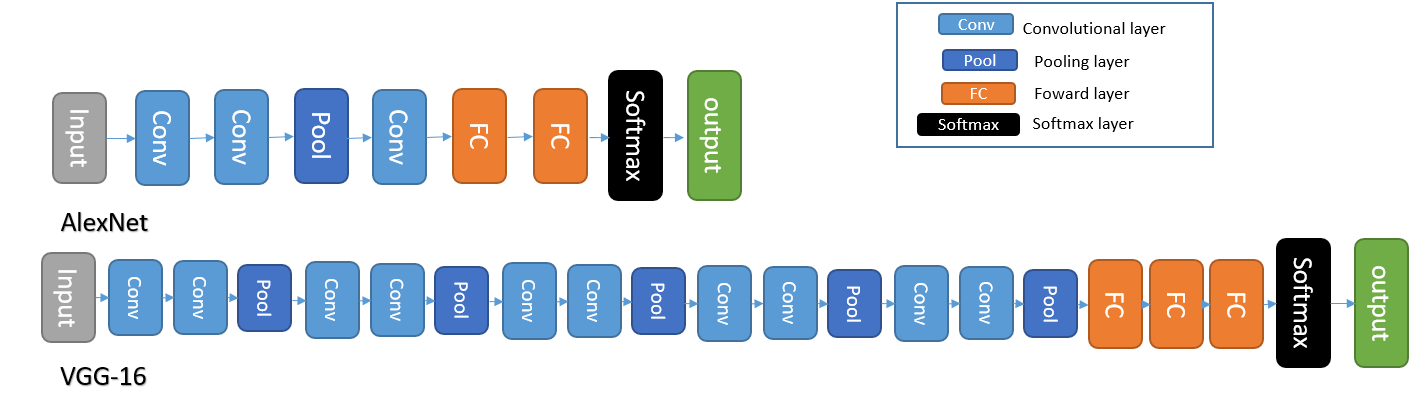
\includegraphics[width=1\columnwidth]{Image/alexvgg.PNG}
\caption[CNNpic1]{ Architecture Comparition between Alexnet and VGG-16  \cite{CNNpic}}
\label{fig:BoxesAndArrowsAreNice}
\end{center}
\end{figure}